\documentclass{article}

    \usepackage{fancyhdr}
    \usepackage{extramarks}
    \usepackage{amsmath}
    \usepackage{amsthm}
    \usepackage{amsfonts}
    \usepackage{tikz}
    \usepackage{amssymb}
    \usepackage{subcaption}
    \usepackage{blkarray}
    \usepackage{algorithm}
    \usepackage{algorithmicx}
    \usepackage{mathtools}
    \usepackage{bm}
    \usepackage{esvect}
    \usepackage{graphicx}
    \usepackage{forest}
    \usepackage{tabulary}
    \usepackage{amsmath}
    \usepackage{algorithm}
    \usepackage{algpseudocode}
    \usepackage[utf8]{inputenc}
    \usepackage{enumerate}
    \usepackage{geometry}
    \usepackage{mathtools}
    \usepackage{parskip}
    \usepackage{xifthen, xparse}
    \usepackage{capt-of}


    \usetikzlibrary{arrows, automata}
    \usetikzlibrary{chains,positioning} %
    \usetikzlibrary{automata,positioning}
    \usetikzlibrary{trees}
    \usepackage[labelformat=empty]{caption}




    

    \makeatletter
    \def\BState{\State\hskip-\ALG@thistlm}
    \makeatother


    \newcommand{\Mod}[1]{\ (\mathrm{mod}\ #1)}

    % \usepackage[newcommands]{ragged2e}


    \usetikzlibrary{trees}

    \newcommand{\question}{\textbf{Question:}}
    \newcommand{\answer}{\textbf{Answer:}}
    \newcommand{\modx}{\;(\bmod\;}

    


    \usetikzlibrary{decorations.markings}
    \tikzstyle{vertex}=[circle, draw, inner sep=0pt, minimum size=6pt]
    \newcommand{\vertex}{\node[vertex]}

    
    

    
    \algdef{SE}[SUBALG]{Indent}{EndIndent}{}{\algorithmicend\ }%
    \algtext*{Indent}
    \algtext*{EndIndent}
    
    
    
    \usetikzlibrary{automata,positioning}
    
    %
    % Basic Document Settings
    %
    
    \topmargin=-0.45in
    \evensidemargin=0in
    \oddsidemargin=0in
    \textwidth=6.5in
    \textheight=9.0in
    \headsep=0.25in
    
    \linespread{1.1}
    
    \pagestyle{fancy}
    \lhead{\hmwkAuthorName}
    \chead{\hmwkClass\ \hmwkTitle}
    \rhead{\firstxmark}
    \lfoot{\lastxmark}
    \cfoot{\thepage}
    
    \renewcommand\headrulewidth{0.4pt}
    \renewcommand\footrulewidth{0.4pt}
    
    \setlength\parindent{0pt}
    
    %
    % Create Problem Sections
    %
    
    \newcommand{\enterProblemHeader}[1]{
        \nobreak\extramarks{}{Problem \arabic{#1} continued on next page\ldots}\nobreak{}
        \nobreak\extramarks{Problem \arabic{#1} (continued)}{Problem \arabic{#1} continued on next page\ldots}\nobreak{}
    }
    
    \newcommand{\exitProblemHeader}[1]{
        \nobreak\extramarks{Problem \arabic{#1} (continued)}{Problem \arabic{#1} continued on next page\ldots}\nobreak{}
        \stepcounter{#1}
        \nobreak\extramarks{Problem \arabic{#1}}{}\nobreak{}
    }
    
    \newcommand\rowop[1]{\scriptstyle\smash{\xrightarrow[\vphantom{#1}]{\mkern-4mu#1\mkern-4mu}}}
    
    \DeclareDocumentCommand\converttorows%
    {>{\SplitList{,}}m}%
    {\ProcessList{#1}{\converttorow}}
    \NewDocumentCommand{\converttorow}{m}
    {\ifthenelse{\isempty{#1}}{}{\rowop{#1}}\\}
    
    \DeclareDocumentCommand \rowops{m}
    {\;
     \begin{matrix}
    \converttorows {#1}
     \end{matrix}
     \; }
    
    \setcounter{secnumdepth}{0}
    \newcounter{partCounter}
    \newcounter{homeworkProblemCounter}
    \setcounter{homeworkProblemCounter}{1}
    \nobreak\extramarks{Problem \arabic{homeworkProblemCounter}}{}\nobreak{}
    
    %
    % Homework Problem Environment
    %
    % This environment takes an optional argument. When given, it will adjust the
    % problem counter. This is useful for when the problems given for your
    % assignment aren't sequential. See the last 3 problems of this template for an
    % example.
    %
    \newenvironment{homeworkProblem}[1][-1]{
        \ifnum#1>0
            \setcounter{homeworkProblemCounter}{#1}
        \fi
        \section{Problem \arabic{homeworkProblemCounter}}
        \setcounter{partCounter}{1}
        \enterProblemHeader{homeworkProblemCounter}
    }{
        \exitProblemHeader{homeworkProblemCounter}
    }
    
    %
    % Homework Details
    %   - Title
    %   - Due date
    %   - Class
    %   - Section/Time
    %   - Instructor
    %   - Author
    %
    
    \newcommand{\hmwkTitle}{SOFTENG211 Assignment \#4}
    \newcommand{\hmwkClass}{S.E. Theory}
    \newcommand{\hmwkAuthorName}{\textbf{Nisarag Bhatt}}

    %
    % Title Page
    %
    
    \title{
        \vspace{2in}
        \textmd{\textbf{\hmwkClass:\ \hmwkTitle}}\\
        \vspace{3in}
    }
    
    \author{\hmwkAuthorName}
    \date{}
    
    \newtheorem{theorem}{Theorem}

    \renewcommand{\part}[1]{\textbf{\large Part \Alph{partCounter}}\stepcounter{partCounter}\\}
    
    %
    % Various Helper Commands
    %
    
    % Useful for algorithms
    \newcommand{\alg}[1]{\textsc{\bfseries \footnotesize #1}}
    
    % For derivatives
    \newcommand{\deriv}[1]{\frac{\mathrm{d}}{\mathrm{d}x} (#1)}
    
    % For partial derivatives
    \newcommand{\pderiv}[2]{\frac{\partial}{\partial #1} (#2)}
    
    % Integral dx
    \newcommand{\dx}{\mathrm{d}x}
    
    % Alias for the Solution section header
    \newcommand{\solution}{\textbf{\large Solution}}
    
    % Probability commands: Expectation, Variance, Covariance, Bias
    \newcommand{\E}{\mathrm{E}}
    \newcommand{\Var}{\mathrm{Var}}
    \newcommand{\Cov}{\mathrm{Cov}}
    \newcommand{\Bias}{\mathrm{Bias}}
    
    \begin{document}

    \maketitle
    
    \pagebreak

    \begin{homeworkProblem}
        
        \question  

        Design an algorithm that given an input string from the alphabet consisting of symbols from PROP, logical connectives $\lor$, $\land$, $\rightarrow$, $\neg$  and the left parenthesis (, and the right parenthesis ), decides if the string is a formula.
        Your algorithm should consist of several lines of instructions written in English.


        \answer

        First we define our alphabet to be $\Sigma = \{p_1,...,p_n,\land, \lor, \neg, \rightarrow, ),( \}$

        Then let $s$ be a string over this alphabet. 

        We also define these formulas below as \textbf{\textit{proper}}, where $p, q \in PROP$

        \begin{itemize}
            \item $\neg(p)$ 
            \item $(p \lor q)$ 
            \item $(p \land q)$
            \item $(p \rightarrow q)$
        \end{itemize}

        The below algorithm will find is $s$ is a formula. 

        Note that in line 9, our string $s$ is reduced. 
        
        Also since we are replacing our proper formula $\psi$ with a proposition $\gamma$ we know that $s'$ is formula if and only if $s$ is a formula. 



        \begin{algorithm}
            \caption{Deciding if a string is a formula}\label{euclid}
            \begin{algorithmic}[1]
              \Procedure{isFormula}{$s$} 
                \If {$s \in PROP$} 
                        \State \textbf{return} $True$
                \Else 
                        \State $\psi \gets$ The first occurrence of a \textit{proper} formula in $s$.
                        \If {such a $\psi$ does not exist}
                            \State \textbf{return} $False$
                        \Else 
                            \State $s' \gets s $ but replace $\psi$ with a new proposition $\gamma$. 
                            \State \textbf{return} $\text{isFormula}(s')$
                        \EndIf
                \EndIf
              \EndProcedure
            \end{algorithmic}
        \end{algorithm}




    \end{homeworkProblem}
    
    \pagebreak

    \begin{homeworkProblem}
        
        \question
        
        Provide a linear time algorithm that given a formula in DNF decides if the formula is satisfiable. If you do not know linear time algorithm (that is, did not take SOFTENG 250 class, then provide an algorithm that checks satisfiability of DNF without going through of all truth assignments of the formula).

        \answer

        Before we begin our algorithm we note that our algorithm takes in a string $f$ which is in the form $$f = a_1 \lor a_2 \lor ... \lor a_n$$ for some $n>0$.

        Where $b_i \in PROP$  and $b_i$ is in the form $(b_1 \land b_2 \land ... \land b_m)$ for some $m>0$.


        \begin{algorithm}
            \caption{Checking if a formula in DNF is satisfiable}\label{euclid}
            \begin{algorithmic}[1]
              \Procedure{DNFSatisfiable}{$f$}\Comment{Size: $f = n$, Note that $f$ is a string containing $n$ sub formulas}
                \For{\text{$a_1$ to $a_n$ subformulas in $f$}} \Comment{$\mathcal{O}(n)$}
                    \If {\text{$a_i$} does not contain a pair of complementary pair of literals $(p \land \neg p)$ where $p \in b_i$}
                        \State \textbf{return} $True$ \Comment {If one subformula is true then the whole formula is satisfiable}
                    \EndIf
                \EndFor
                \State 
                \State \textbf{return} $False$ \Comment {If all subformulas have a complementary pair of literals}
              \EndProcedure
            \end{algorithmic}
        \end{algorithm}

        Note that this algorithm is linear because at most you have to check $n$ subformulas hence the algorithm runs in $\mathcal{O}(n)$ time. 

        You only return false when all formulas $(a_1, ... , a_n)$ evaluate are false. 

                
        
           
    \end{homeworkProblem}
    
    \pagebreak

    \begin{homeworkProblem}
        
        \question  

        Consider the following formula:

        $$ (((p \lor (\neg s \rightarrow q)) \land ((q \land s) \lor \neg p)) \rightarrow (\neg s \land q)) $$ 

        Do the following:

        (a) Write down the labeled tree representation of the formula. \\
        (b) Write down the truth table for the formula. \\
        (c) Find a DNF formula equivalent to it.


        \answer

        (a)

        \begin{center} 
            \begin{forest}
                for tree={circle,draw}
                [$\rightarrow$
                    [$\land$
                        [$\lor$
                            [$p$]
                            [$\rightarrow$
                                [$\neg$
                                    [$s$]]
                                [$q$]]
                        ]
                        [$\lor$
                            [$\land$
                                [$q$]
                                [$s$]]
                            [$\neg$
                                [$p$]]
                        ]
                    ]
                    [$\land$
                        [$\neg$
                            [$s$]]
                        [$q$]
                    ]
                ]
            \end{forest}
        \end{center}
 

        (b) 
        First we shall simplify the formula: $ (((p \lor (\neg s \rightarrow q)) \land ((q \land s) \lor \neg p)) \rightarrow (\neg s \land q)) $


        Note that: $(p \lor (\neg s \rightarrow q)) =  (p \lor s \lor q)$ 

        Hence 
        \begin{align*}
            f &= (((p \lor (\neg s \rightarrow q)) \land ((q \land s) \lor \neg p)) \rightarrow (\neg s \land q)) \\
            &= (((p \lor s \lor q) \land ((q \land s) \lor \neg p)) \rightarrow (\neg s \land q)) \\ 
            &= (( (s \land q) \lor (s \land \neg p) \lor (\neg p \land q)) \rightarrow (\neg s \land q)) \\ 
            &= \neg ( (s \land q) \lor (s \land \neg p) \lor (\neg p \land q)) \lor (\neg s \land q) \\ 
            &= ((\neg s \land p) \lor (\neg s \land \neg q) \lor (p \land \neg q) \lor (\neg s \land q)) \\ 
            &= \neg s \lor (p \land \neg q)
        \end{align*}

        \begin{displaymath}  % start unumbered math environment
            %
            % Start a table in math mode.  The |c|c|c|c|c|c|c|c| string is a
            % format string that says there will be 8 colunms in the table.  The
            % c's indicate that the data in each column will be centered (use l
            % for left justified and r for right justified).  The vertical bar
            % means that lines will be drawn between columns.  The trailing
            % \hline causes a horizontal line to be drawn across the top of the
            % table.
            %
            \begin{array}{|c|c|c|c|}\hline
              %
              % Each row of the table consists of data separated by "&" symbols.
              % Each row must end with "\\" to cause a newline.  A trailing
              % \hline will cause a line to be drawn under the row.  A double
              % \hline is often used to separate the table header from the rest
              % of the table. 
              %
              p & q & s & \neg s \lor (p \land \neg q) \\ \hline\hline
              T & T & T & F \\\hline
              T & T & F & T \\\hline
              T & F & T & T \\\hline
              T & F & F & T \\\hline
              F & T & T & F \\\hline
              F & T & F & T \\\hline
              F & F & T & F \\\hline
              F & F & F & T \\\hline
            \end{array}
          \end{displaymath}

          (c) Reading from the truth table, we get that the disjunctive normal form of the formula is:
        $$ DNF = ((p \land q \land \neg s) \lor (p \land \neg q \land s) \lor (p \land \neg q \land \neg s) \lor (\neg p \land q \land \neg s) \lor (\neg p \land \neg q \land \neg s))$$
          
        
    
    
    \end{homeworkProblem}
    
    \pagebreak

    \begin{homeworkProblem}
        
        \question 

        Write down all languages over two letter alphabet $\{a, b\}$ recognised by two state DFA.

        \answer

        I have expressed the languages in regular expressions since it is much easier to write.

        All answers assume $w \in \{a, b\}^{*}$ and note that $\lambda = \text{the empty string}$

        The reasoning behind how there are 26 languages is as follows:

        We start with a two state DFA which contains two states $Q = \{q_0, q_1\}$. This DFA is over the binary alphabet $\Sigma = \{a,b\}$.

        Note that the transition function is as follows : 
        \begin{align*}
            \delta &: Q \times \Sigma \rightarrow Q  \\
            \delta(q_0, a) &= ~ q \in Q \\ 
            \delta(q_0, b) &= ~ q \in Q \\
            \delta(q_1, a) &= ~ q \in Q \\
            \delta(q_1, b) &= ~ q \in Q \\
        \end{align*}
        
        Since there are $2$ options for $q \in Q$ and there are $4$ places to place these options there are $2^4=16$ ways to arrange $q_1,q_0$ between the $4$ transitions. This means there are $16$ possible transition functions and hence $16$ DFA's possible for a $2$ state DFA over a binary alphabet.

        However, these specific transitions are disconnected: 

        \begin{center}
            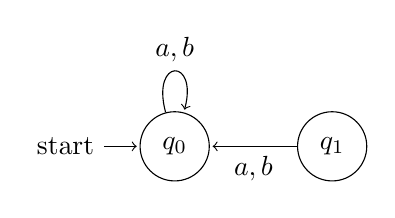
\begin{tikzpicture}[shorten >=1pt,node distance=2cm,on grid,auto] 
                \node[state,initial] (q_0)   {$q_0$}; 
                \node[state] [right=of q_0] (q_1) {$q_1$};
                \path[->] 
                (q_0) edge [loop above] node {$a,b$} ()
                (q_1) edge node {$a,b$} (q_0);
             \end{tikzpicture}
        \end{center}

        \begin{center}
            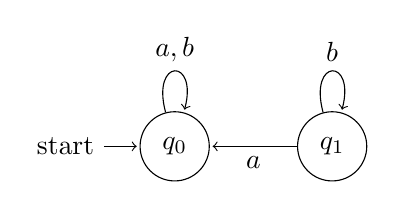
\begin{tikzpicture}[shorten >=1pt,node distance=2cm,on grid,auto] 
                \node[state,initial] (q_0)   {$q_0$}; 
                \node[state] [right=of q_0] (q_1) {$q_1$};
                \path[->] 
                (q_0) edge [loop above] node {$a,b$} ()
                (q_1) edge [loop above] node {$b$} ()
                      edge node {$a$} (q_0);
             \end{tikzpicture}
        \end{center}

        \begin{center}
            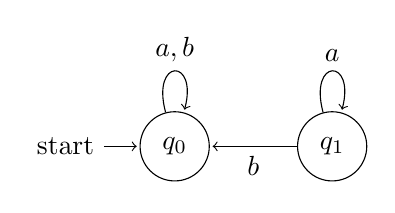
\begin{tikzpicture}[shorten >=1pt,node distance=2cm,on grid,auto] 
                \node[state,initial] (q_0)   {$q_0$}; 
                \node[state] [right=of q_0] (q_1) {$q_1$};
                \path[->] 
                (q_0) edge [loop above] node {$a,b$} ()
                (q_1) edge [loop above] node {$a$} ()
                      edge node {$b$} (q_0);
             \end{tikzpicture}
        \end{center}

        \begin{center}
            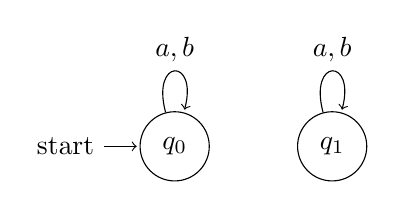
\begin{tikzpicture}[shorten >=1pt,node distance=2cm,on grid,auto] 
                \node[state,initial] (q_0)   {$q_0$}; 
                \node[state] [right=of q_0] (q_1) {$q_1$};
                \path[->] 
                (q_0) edge [loop above] node {$a,b$} ()
                (q_1) edge [loop above] node {$a,b$} ();
             \end{tikzpicture}
        \end{center}

        These 4 transition functions were function in which the initial state could not reach the second state, so effectively there was only one possible state so it they are trivial to analyse:

        Hence there are only 12 transitions to consider.
        Now, since there are two states : $q_0, q_1$ there are $2^2$ = $4$ ways to pick which ones are accepting and which are non accepting. Namely these are:  

        \begin{displaymath}  
            \begin{array}{|c||c|c|}\hline
            \text{Case} & q_0 & q_1 \\ \hline\hline
            1 & \text{Accepting} & \text{Accepting} \\\hline
            2 & \text{Accepting} & \text{Not Accepting} \\\hline
            3 & \text{Not Accepting} & \text{Accepting} \\\hline
            4 & \text{Not Accepting} & \text{Not Accepting} \\\hline
            \end{array}
        \end{displaymath}

        For each possible case there are $16$ different possible transitions. Which means for each case there are $16$ languages however one may observe that:

        \begin{itemize}
            \item For case $1$, both $q_0$ and $q_1$ are accepting which means there is only one possible language since it doesn't matter what transitions exist in the transition function because any of them will give the same language. Hence we can reduce the number of languages for this case from $16 \to 1$. 
            \item For case $2$, we need to analyse $12$ transition functions. Hence the number of languages for this case is $12$. 
            \item For case $3$, we need to analyse $12$ transition functions. Hence the number of languages for this case is $12$. 
            \item For case $4$, both $q_0$ and $q_1$ are not accepting which means there is effectively no language for this DFA so any transition function will result in the empty set. Hence we can reduce the number of languages for this case from $16 \to 1$. 
        \end{itemize}

        Therefore the total number of languages must be $12+12+1+1=26$.

        Below, I have shown all the DFA's corresponding to the $26$ possible languages and expressed the languages in a regular expression form. 

        \begin{center}
            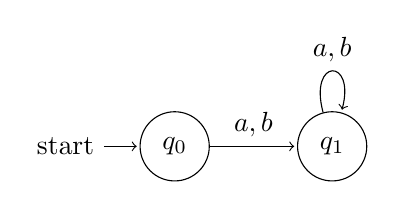
\begin{tikzpicture}[shorten >=1pt,node distance=2cm,on grid,auto] 
                \node[state,initial] (q_0)   {$q_0$}; 
                \node[state] [right=of q_0] (q_1) {$q_1$};
                \path[->] 
                (q_0) edge node {$a,b$} (q_1)
                (q_1) edge [loop above] node {$a,b$} ();
            \end{tikzpicture}
            \captionof{figure}{Language is $L_0 = \phi = \{ \} $ (Doesn't matter what our transition is since there is no accepting state)}
        \end{center}

        \begin{center}
            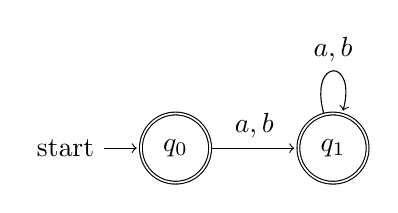
\begin{tikzpicture}[shorten >=1pt,node distance=2cm,on grid,auto] 
                \node[state,initial, accepting] (q_0)   {$q_0$}; 
                \node[state, accepting] [right=of q_0] (q_1) {$q_1$};
                \path[->] 
                (q_0) edge node {$a,b$} (q_1)
                (q_1) edge [loop above] node {$a,b$} ();
            \end{tikzpicture}
            \captionof{figure}{Language is $L_1 = \{w | w ~ \text{is in the form} ~ (a+b)^{\star}\}$ (Any transitions resulting in this regular expression)}
        \end{center}

        \begin{center}
            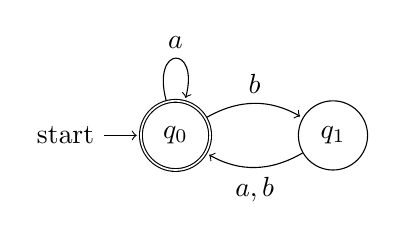
\begin{tikzpicture}[shorten >=1pt,node distance=2cm,on grid,auto] 
                \node[state,initial, accepting] (q_0)   {$q_0$}; 
                \node[state] [right=of q_0] (q_1) {$q_1$};
                \path[->] 
                (q_0) edge [loop above] node {$a$} ()
                        edge [bend left, above] node {$b$} (q_1)
                (q_1) edge [bend left, below] node {$a,b$} (q_0);
            \end{tikzpicture}
            \captionof{figure}{Language is $L_2 = \{w | w ~ \text{is in the form} ~ (a+b(a+b))^{\star}\}$}
        \end{center}


        \begin{center}
            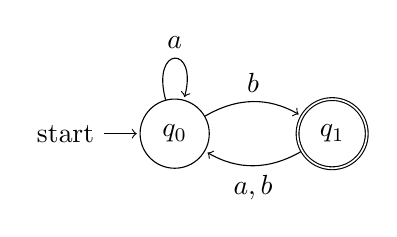
\begin{tikzpicture}[shorten >=1pt,node distance=2cm,on grid,auto] 
                \node[state,initial] (q_0)   {$q_0$}; 
                \node[state, accepting] [right=of q_0] (q_1) {$q_1$};
                \path[->] 
                (q_0) edge [loop above] node {$a$} ()
                        edge [bend left, above] node {$b$} (q_1)
                (q_1) edge [bend left, below] node {$a,b$} (q_0);
            \end{tikzpicture}
            \captionof{figure}{Language is $L_3 = \{w | w ~ \text{is in the form} ~ (a+b(a+b))^{\star}b \}$}
        \end{center}

        \begin{center}
            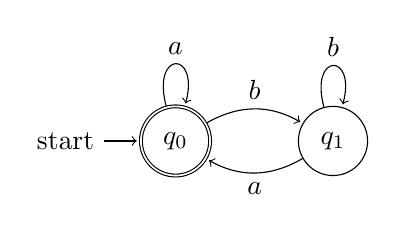
\begin{tikzpicture}[shorten >=1pt,node distance=2cm,on grid,auto] 
                \node[state,initial, accepting] (q_0)   {$q_0$}; 
                \node[state] [right=of q_0] (q_1) {$q_1$};
                \path[->] 
                (q_0) edge [loop above] node {$a$} ()
                        edge [bend left, above] node {$b$} (q_1)
                (q_1) edge [bend left, below] node {$a$} (q_0)
                    edge [loop above] node {$b$} ();
            \end{tikzpicture}
            \captionof{figure}{Language is $L_4 = \{w | w ~ \text{is in the form} ~ (a+bb^{\star}a)^{\star} \}$}
        \end{center}

        \begin{center}
            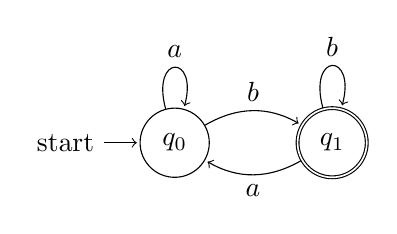
\begin{tikzpicture}[shorten >=1pt,node distance=2cm,on grid,auto] 
                \node[state,initial] (q_0)   {$q_0$}; 
                \node[state, accepting] [right=of q_0] (q_1) {$q_1$};
                \path[->] 
                (q_0) edge [loop above] node {$a$} ()
                        edge [bend left, above] node {$b$} (q_1)
                (q_1) edge [bend left, below] node {$a$} (q_0)
                    edge [loop above] node {$b$} ();
            \end{tikzpicture}
            \captionof{figure}{Language is $L_5 = \{w | w ~ \text{is in the form} ~ (a+bb^{\star}a)^{\star}bb^{\star}\}$}
        \end{center}

        \begin{center}
            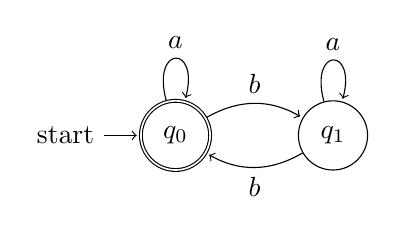
\begin{tikzpicture}[shorten >=1pt,node distance=2cm,on grid,auto] 
                \node[state,initial, accepting] (q_0)   {$q_0$}; 
                \node[state] [right=of q_0] (q_1) {$q_1$};
                \path[->] 
                (q_0) edge [loop above] node {$a$} ()
                        edge [bend left, above] node {$b$} (q_1)
                (q_1) edge [bend left, below] node {$b$} (q_0)
                    edge [loop above] node {$a$} ();
            \end{tikzpicture}
            \captionof{figure}{Language is $L_6 = \{w | w ~ \text{is in the form} ~ (a+ba^{\star}b)^{\star} \}$}
        \end{center}

        \begin{center}
            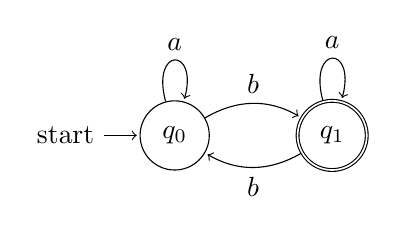
\begin{tikzpicture}[shorten >=1pt,node distance=2cm,on grid,auto] 
                \node[state,initial] (q_0)   {$q_0$}; 
                \node[state, accepting] [right=of q_0] (q_1) {$q_1$};
                \path[->] 
                (q_0) edge [loop above] node {$a$} ()
                        edge [bend left, above] node {$b$} (q_1)
                (q_1) edge [bend left, below] node {$b$} (q_0)
                    edge [loop above] node {$a$} ();
            \end{tikzpicture}
            \captionof{figure}{Language is $L_7 = \{w | w ~ \text{is in the form} ~ (a+ba^{\star}b)^{\star}ba^{\star} \}$}
        \end{center}

        \begin{center}
            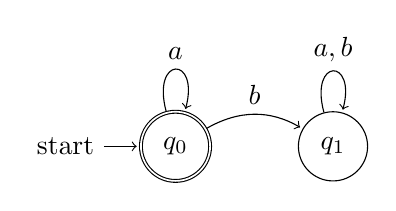
\begin{tikzpicture}[shorten >=1pt,node distance=2cm,on grid,auto] 
                \node[state,initial, accepting] (q_0)   {$q_0$}; 
                \node[state] [right=of q_0] (q_1) {$q_1$};
                \path[->] 
                (q_0) edge [loop above] node {$a$} ()
                        edge [bend left, above] node {$b$} (q_1)
                (q_1) edge [loop above] node {$a,b$} ();
            \end{tikzpicture}
            \captionof{figure}{Language is $L_8 = \{w | w ~ \text{is in the form} ~ a^{\star} \}$}
        \end{center}

        \begin{center}
            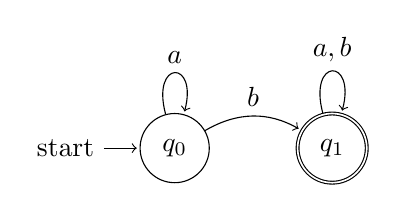
\begin{tikzpicture}[shorten >=1pt,node distance=2cm,on grid,auto] 
                \node[state,initial] (q_0)   {$q_0$}; 
                \node[state, accepting] [right=of q_0] (q_1) {$q_1$};
                \path[->] 
                (q_0) edge [loop above] node {$a$} ()
                        edge [bend left, above] node {$b$} (q_1)
                (q_1) edge [loop above] node {$a,b$} ();
            \end{tikzpicture}
            \captionof{figure}{Language is $L_9 = \{w | w ~ \text{is in the form} ~ a^{\star}b(a+b)^{\star} \}$}
        \end{center}

        \begin{center}
            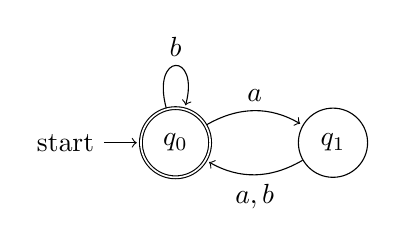
\begin{tikzpicture}[shorten >=1pt,node distance=2cm,on grid,auto] 
                \node[state,initial, accepting] (q_0)   {$q_0$}; 
                \node[state] [right=of q_0] (q_1) {$q_1$};
                \path[->] 
                (q_0) edge [loop above] node {$b$} ()
                        edge [bend left, above] node {$a$} (q_1)
                (q_1) edge [bend left, below] node {$a,b$} (q_0);
            \end{tikzpicture}
            \captionof{figure}{Language is $L_{10} = \{w | w ~ \text{is in the form} ~ (b+a(a+b))^{\star}     \}$}
        \end{center}

        \begin{center}
            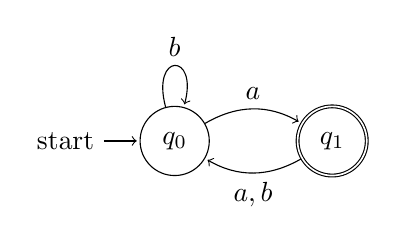
\begin{tikzpicture}[shorten >=1pt,node distance=2cm,on grid,auto] 
                \node[state,initial] (q_0)   {$q_0$}; 
                \node[state, accepting] [right=of q_0] (q_1) {$q_1$};
                \path[->] 
                (q_0) edge [loop above] node {$b$} ()
                        edge [bend left, above] node {$a$} (q_1)
                (q_1) edge [bend left, below] node {$a,b$} (q_0);
            \end{tikzpicture}
            \captionof{figure}{Language is $L_{11} = \{w | w ~ \text{is in the form} ~ (b+a(a+b))^{\star}a     \}$}
        \end{center}

        \begin{center}
            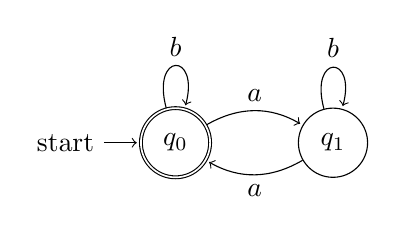
\begin{tikzpicture}[shorten >=1pt,node distance=2cm,on grid,auto] 
                \node[state,initial, accepting] (q_0)   {$q_0$}; 
                \node[state] [right=of q_0] (q_1) {$q_1$};
                \path[->] 
                (q_0) edge [loop above] node {$b$} ()
                        edge [bend left, above] node {$a$} (q_1)
                (q_1) edge [bend left, below] node {$a$} (q_0)
                    edge [loop above] node {$b$} ();
            \end{tikzpicture}
            \captionof{figure}{Language is $L_{12} = \{w | w ~ \text{is in the form} ~  (b+ab^{\star}a)^{\star}     \}$}
        \end{center}

        \begin{center}
            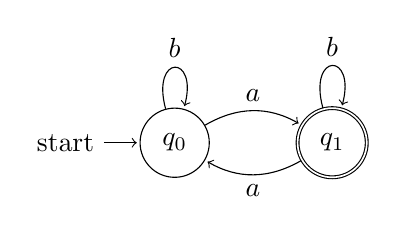
\begin{tikzpicture}[shorten >=1pt,node distance=2cm,on grid,auto] 
                \node[state,initial] (q_0)   {$q_0$}; 
                \node[state, accepting] [right=of q_0] (q_1) {$q_1$};
                \path[->] 
                (q_0) edge [loop above] node {$b$} ()
                        edge [bend left, above] node {$a$} (q_1)
                (q_1) edge [bend left, below] node {$a$} (q_0)
                    edge [loop above] node {$b$} ();
            \end{tikzpicture}
            \captionof{figure}{Language is $L_{13} = \{w | w ~ \text{is in the form} ~  (b+ab^{\star}a)^{\star}ab^{\star} \}$}
        \end{center}

        \begin{center}
            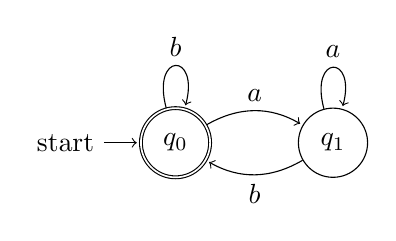
\begin{tikzpicture}[shorten >=1pt,node distance=2cm,on grid,auto] 
                \node[state,initial, accepting] (q_0)   {$q_0$}; 
                \node[state] [right=of q_0] (q_1) {$q_1$};
                \path[->] 
                (q_0) edge [loop above] node {$b$} ()
                        edge [bend left, above] node {$a$} (q_1)
                (q_1) edge [bend left, below] node {$b$} (q_0)
                    edge [loop above] node {$a$} ();
            \end{tikzpicture}
            \captionof{figure}{Language is $L_{14} = \{w | w ~ \text{is in the form} ~  (b+aa^{\star}b)^{\star} \}$}
        \end{center}

        \begin{center}
            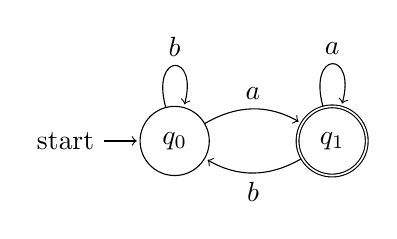
\begin{tikzpicture}[shorten >=1pt,node distance=2cm,on grid,auto] 
                \node[state,initial] (q_0)   {$q_0$}; 
                \node[state, accepting] [right=of q_0] (q_1) {$q_1$};
                \path[->] 
                (q_0) edge [loop above] node {$b$} ()
                        edge [bend left, above] node {$a$} (q_1)
                (q_1) edge [bend left, below] node {$b$} (q_0)
                    edge [loop above] node {$a$} ();
            \end{tikzpicture}
            \captionof{figure}{Language is $L_{15} = \{w | w ~ \text{is in the form} ~  (b+aa^{\star}b)^{\star}aa^{\star}     \}$}
        \end{center}

        \pagebreak

        \begin{center}
            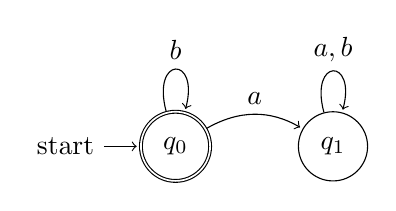
\begin{tikzpicture}[shorten >=1pt,node distance=2cm,on grid,auto] 
                \node[state,initial, accepting] (q_0)   {$q_0$}; 
                \node[state] [right=of q_0] (q_1) {$q_1$};
                \path[->] 
                (q_0) edge [loop above] node {$b$} ()
                        edge [bend left, above] node {$a$} (q_1)
                (q_1) edge [loop above] node {$a,b$} ();
            \end{tikzpicture}
            \captionof{figure}{Language is $L_{16} = \{w | w ~ \text{is in the form} ~   b^{\star}     \}$}
        \end{center}

        \begin{center}
            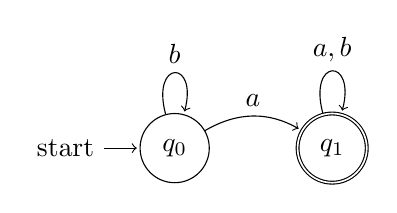
\begin{tikzpicture}[shorten >=1pt,node distance=2cm,on grid,auto] 
                \node[state,initial] (q_0)   {$q_0$}; 
                \node[state, accepting] [right=of q_0] (q_1) {$q_1$};
                \path[->] 
                (q_0) edge [loop above] node {$b$} ()
                        edge [bend left, above] node {$a$} (q_1)
                (q_1) edge [loop above] node {$a,b$} ();
            \end{tikzpicture}
            \captionof{figure}{Language is $L_{17} = \{w | w ~ \text{is in the form} ~    b^{\star}a(b+a)^{\star}     \}$}
        \end{center}

        \begin{center}
            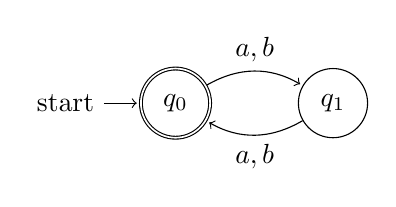
\begin{tikzpicture}[shorten >=1pt,node distance=2cm,on grid,auto] 
                \node[state,initial, accepting] (q_0)   {$q_0$}; 
                \node[state] [right=of q_0] (q_1) {$q_1$};
                \path[->] 
                (q_0) edge [bend left, above] node {$a,b$} (q_1)
                (q_1) edge [bend left, below] node {$a,b$} (q_0);
            \end{tikzpicture}
            \captionof{figure}{Language is $L_{18} = \{w | w ~ \text{is in the form} ~    ((b+a)(b+a))^{\star}     \}$}
        \end{center}

        \begin{center}
            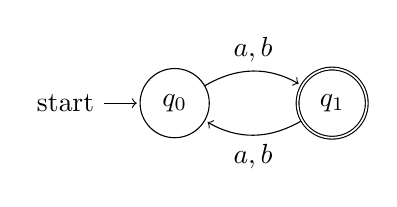
\begin{tikzpicture}[shorten >=1pt,node distance=2cm,on grid,auto] 
                \node[state,initial] (q_0)   {$q_0$}; 
                \node[state, accepting] [right=of q_0] (q_1) {$q_1$};
                \path[->] 
                (q_0) edge [bend left, above] node {$a,b$} (q_1)
                (q_1) edge [bend left, below] node {$a,b$} (q_0);
            \end{tikzpicture}
            \captionof{figure}{Language is $L_{19} = \{w | w ~ \text{is in the form} ~    ((b+a)(b+a))^{\star}(b+a)     \}$}
        \end{center}

        \begin{center}
            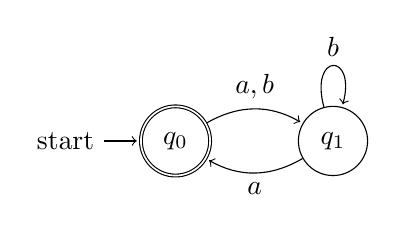
\begin{tikzpicture}[shorten >=1pt,node distance=2cm,on grid,auto] 
                \node[state,initial, accepting] (q_0)   {$q_0$}; 
                \node[state] [right=of q_0] (q_1) {$q_1$};
                \path[->] 
                (q_0) edge [bend left, above] node {$a,b$} (q_1)
                (q_1) edge [bend left, below] node {$a$} (q_0)
                    edge [loop above] node {$b$} ();
            \end{tikzpicture}
            \captionof{figure}{Language is $L_{20} = \{w | w ~ \text{is in the form} ~    ((a+b)b^{\star}a)^{\star}     \}$}
        \end{center}

        \begin{center}
            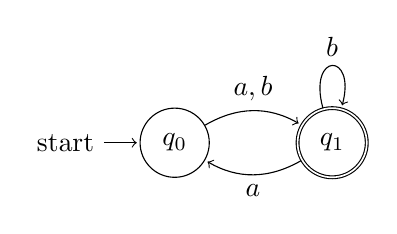
\begin{tikzpicture}[shorten >=1pt,node distance=2cm,on grid,auto] 
                \node[state,initial] (q_0)   {$q_0$}; 
                \node[state, accepting] [right=of q_0] (q_1) {$q_1$};
                \path[->] 
                (q_0) edge [bend left, above] node {$a,b$} (q_1)
                (q_1) edge [bend left, below] node {$a$} (q_0)
                    edge [loop above] node {$b$} ();
            \end{tikzpicture}
            \captionof{figure}{Language is $L_{21} = \{w | w ~ \text{is in the form} ~ ((a+b)b^{\star}a)^{\star}(a+b)b^{\star}(b+\lambda)        \}$}
        \end{center}

        \begin{center}
            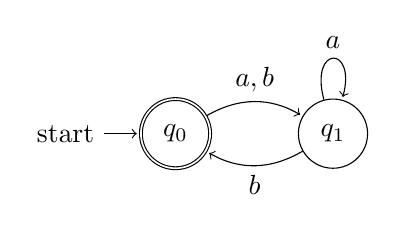
\begin{tikzpicture}[shorten >=1pt,node distance=2cm,on grid,auto] 
                \node[state,initial, accepting] (q_0)   {$q_0$}; 
                \node[state] [right=of q_0] (q_1) {$q_1$};
                \path[->] 
                (q_0) edge [bend left, above] node {$a,b$} (q_1)
                (q_1) edge [bend left, below] node {$b$} (q_0)
                    edge [loop above] node {$a$} ();
            \end{tikzpicture}
            \captionof{figure}{Language is $L_{22} = \{w | w ~ \text{is in the form} ~ ((a+b)a^{\star}b)^{\star}       \}$}
        \end{center}

        \begin{center}
            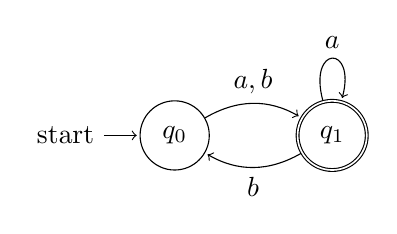
\begin{tikzpicture}[shorten >=1pt,node distance=2cm,on grid,auto] 
                \node[state,initial] (q_0)   {$q_0$}; 
                \node[state, accepting] [right=of q_0] (q_1) {$q_1$};
                \path[->] 
                (q_0) edge [bend left, above] node {$a,b$} (q_1)
                (q_1) edge [bend left, below] node {$b$} (q_0)
                    edge [loop above] node {$a$} ();
            \end{tikzpicture}
            \captionof{figure}{Language is $L_{23} = \{w | w ~ \text{is in the form} ~ ((a+b)a^{\star}b)^{\star}(a+b)a^{\star}(a+\lambda)      \}$}
        \end{center}

        \begin{center}
            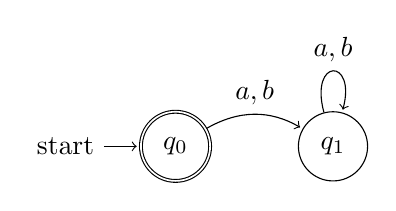
\begin{tikzpicture}[shorten >=1pt,node distance=2cm,on grid,auto] 
                \node[state,initial, accepting] (q_0)   {$q_0$}; 
                \node[state] [right=of q_0] (q_1) {$q_1$};
                \path[->] 
                (q_0) edge [bend left, above] node {$a,b$} (q_1)
                (q_1) edge [loop above] node {$a,b$} ();
            \end{tikzpicture}
            \captionof{figure}{Language is $L_{24} = \{w | w ~ \text{is in the form} ~  \lambda      \}$}
        \end{center}

        \begin{center}
            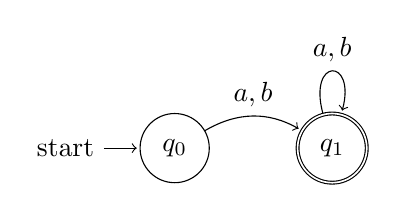
\begin{tikzpicture}[shorten >=1pt,node distance=2cm,on grid,auto] 
                \node[state,initial] (q_0)   {$q_0$}; 
                \node[state, accepting] [right=of q_0] (q_1) {$q_1$};
                \path[->] 
                (q_0) edge [bend left, above] node {$a,b$} (q_1)
                (q_1) edge [loop above] node {$a,b$} ();
            \end{tikzpicture}
            \captionof{figure}{Language is $L_{25} = \{w | w ~ \text{is in the form} ~ (a+b)(b+a)^{\star}(b+a+ \lambda)         \}$}
        \end{center}


    \end{homeworkProblem}
    
    \pagebreak

    \begin{homeworkProblem}
        
        \question  

        Let $L$ be a language over the alphabet $\{a, b, c\}$ recognised by NFA. Consider the language $L'$ such that every string $w' \in L'$
        is obtained from a string $w \in L$ by replacing all occurrences of $c$ in $w$ by $a$. Prove that $L'$ is NFA recognizable. 


        \answer

        \begin{proof}
            Consider a NFA: $\mathcal{M}$ which recognizes $L$. To complete this proof we must prove that there exists an NFA: $\mathcal{M'}$ in which $\mathcal{M'}$ recognizes $L'$.
    
            First, we construct $\mathcal{M'}$ by taking $\mathcal{M}$ and considering all the transitions of $\mathcal{M}$. For the transitions that are labelled $c$, replace $c$ with $a$. By doing this we produce a language $L(\mathcal{M}') $. 
    
            To complete this proof, it suffices to show that $L(\mathcal{M}') = L'$ 
    
            \begin{proof}
                Prove that:  $L' \subseteq L(\mathcal{M}')$ 
    
                Consider a string $w' \in L'$. By the definition of how $L'$ was constructed there must exist a $w \in L$ in which $w'$ is constructed by replacing all occurrences of $c$ in $w$ by $a$.
    
                From this we must know that there exists an accepting \textit{run} in $\mathcal{M}$ for the string $w$. Since we constructed $\mathcal{M}$ by replacing all transitions that are labelled $c$ with $a$, this means the accepting run is preserved since anytime $\mathcal{M'}$ processes a $c$, $\mathcal{M'}$ will behave the same way as $\mathcal{M}$. (I.e. there is an accepting run of $\mathcal{M'}$ on $w'$)
                
                This must mean that $w' \in L(\mathcal{M'})$ and because $w'$ was picked arbitrarily, this argument works for any string ($w' \in L'$). This means that $L' \subseteq L(\mathcal{M}')$. 
            \end{proof}
    
            \begin{proof}
                Prove that:  $L(\mathcal{M}') \subseteq L'$ 
    
                We once again consider a string $w' \in L(\mathcal{M}')$. Consider an accepting run for $w'$ by $\mathcal{M'}$, call this run $\zeta$. 
    
                We will now take $w'$, we then construct a new string $w$ by taking $w'$ and replacing an occurrence of $a$ with $c$  when $\zeta$ goes through a transition which would have been labelled by $c$ in $\mathcal{M}$.
    
                Now $\mathcal{M}$ will have an accepting run for $w$ and because of this $w \in L$. Since we can make $w'$ again by taking $w$ and replacing all occurrences of $c$ with $a$.
                
                This must mean that $w' \in L'$. Hence,  $L(\mathcal{M}') \subseteq L'$. 
    
            \end{proof}
            
            Since  $L' \subseteq L(\mathcal{M}')$  and  $L(\mathcal{M}') \subseteq L'$, it must mean that $L(\mathcal{M}') = L'$. This means that $L'$ is NFA recognizable since it is a language recognized by the NFA $\mathcal{M'}$.
            
        \end{proof}
        
        
    \end{homeworkProblem}
    
    \pagebreak

    \begin{homeworkProblem}
        
        \question 
        
        Over the alphabet $\{a, b\}$, consider the language $L = \{w | ~ \text{the string}  ~ w ~ \text{starts with an} ~ a\}$. Prove that no DFA with two states recognises L.

        \answer

        We shall prove this by contradiction:

        \begin{proof}
            Assume that there does exists a two state DFA that recognises $L = \{w | ~ \text{the string}  ~ w ~ \text{starts with an} ~ a\}$ over the alphabet $\Sigma = \{a, b\}$. 

            We first note that a two state $S = (q_0, q_1)$ DFA over a binary alphabet must contain $4$ transitions because $S \times \Sigma = \{(q_0, a), (q_0, b), (q_1, a), (q_1, b)\}$

            Now we begin by construction 

            We start of with one state: 
            
            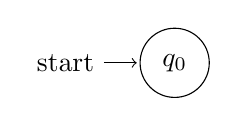
\begin{tikzpicture}[shorten >=1pt,node distance=2cm,on grid,auto] 
                \node[state,initial] (q_0)   {$q_0$}; 
            \end{tikzpicture}

            If a string $w$ begins with an $a$ then when $q_0$ receives an $a$ from a string it \textit{must} go into an accepting state $(q_1)$ so we have a transition $(q_0, a)=q_1$: 

            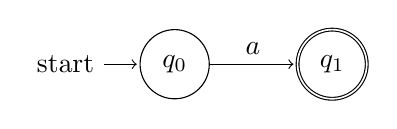
\begin{tikzpicture}[shorten >=1pt,node distance=2cm,on grid,auto] 
                \node[state,initial] (q_0)   {$q_0$};
                \node[state,accepting] [right=of q_0] (q_1) {$q_1$}; 
                \path[->]
                (q_0) edge node {$a$} (q_1);
            \end{tikzpicture}

            When in the accepting state $(q_1)$, if it receives either $a$ or $b$ it has to stay \textit{accepted} because you can't go back to a not accepting state $(q_0)$ since $w$ already started with $a$ so it must be accepting. 
            
            So we must have two more transitions $(q_1, a)=q_1$ and $(q_1, b)=q_1$. 

            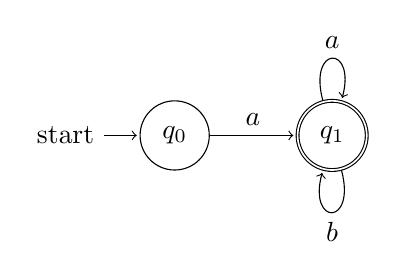
\begin{tikzpicture}[shorten >=1pt,node distance=2cm,on grid,auto] 
                \node[state,initial] (q_0)   {$q_0$};
                \node[state,accepting] [right=of q_0] (q_1) {$q_1$}; 
                \path[->]
                (q_0) edge node {$a$} (q_1)
                (q_1) edge [loop above] node {$a$} ()
                (q_1) edge [loop below] node {$b$} ();
            \end{tikzpicture}

            We have now used $3$ of our transitions: since we used $(q_0, a)=q_1, (q_1, a)=q_1, (q_1, b)=q_1$. The remaining transition is $(q_0, b)$. 

            The only states the transition  $(q_0, b)$ can go to is either $(q_0,b)=q_0$ or $(q_0, b)=q_1$

            If $(q_0,b)=q_0$ then that means if a string that contains a $b$ stays in the same state $(q_0)$. However this would mean a string such as $"ba"$ is accepted because when you begin the DFA you start at $q_0$ then you process a $b$ : $(q_0,b)=q_0$, after you process an $a$ : $(q_0,a)=q_1$ you end up in $q_1$ 
            which means the string $"ba"$ is accepted. However this string does \textit{not} start with $a$ so we can't have the transition: $(q_0,b)=q_0$. 

            If $(q_0,b)=q_1$ then that means a string such as $"b"$ is accepted however this can't be the case because only strings that begin with $a$ are accepted. 

            Since we can't have either $(q_0,b)=q_0$ and $(q_0, b)=q_1$ we must require atleast another state for $(q_0,b)$ to transition to. Therefore contradiction.             Hence, we cannot construct a DFA with two states that recognises L.
        \end{proof}
        
    \end{homeworkProblem}
    
    \pagebreak

    \begin{homeworkProblem}
        
        \question  

        Over the alphabet $\{a, b\}$, consider the languages $L_1 = \{w | \text{the string $w$ starts with an $a$} \} $ and 
        
        $L_2 =\{w|\text{the number of symbols $b$ in $w$ is $1$ modulo $3$}\}$. Do the following:


        \begin{itemize}
            \item Draw diagrams for DFA recognising both $L_1$ and $L_2$.
            \item Draw a diagram for DFA recognising $L_1 \cap L_2$.
        \end{itemize}
        
        \answer

        \begin{center}
    
            $L_1 = \{w | \text{the string $w$ starts with an $a$} \}$

            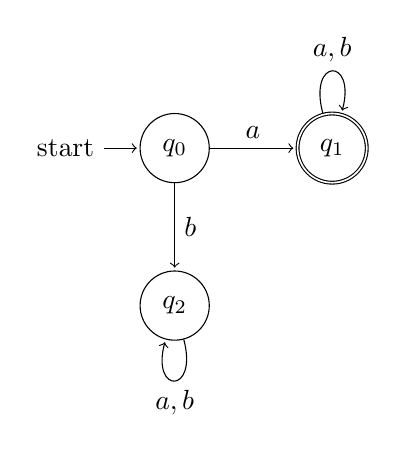
\begin{tikzpicture}[shorten >=1pt,node distance=2cm,on grid,auto] 
                \node[state,initial] (q_0)   {$q_0$}; 
                \node[state, accepting] [right=of q_0] (q_1) {$q_1$};
                \node[state](q_2) [below =of q_0] {$q_2$};
                \path[->] 
                (q_0) edge node {$a$} (q_1)
                      edge node {$b$} (q_2)
                (q_1) edge [loop above] node {$a,b$} ()
                (q_2) edge [loop below] node {$a,b$} ();
             \end{tikzpicture}
        \end{center}

       
        \begin{center}
    
            $L_2 =\{w ~ | ~ \text{the number of symbols $b$ in $w$ is $1$ modulo $3$}\}$

            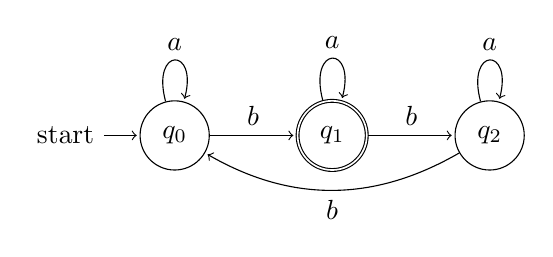
\begin{tikzpicture}[shorten >=1pt,node distance=2cm,on grid,auto] 
                \node[state,initial] (q_0)   {$q_0$}; 
                \node[state,accepting] [right=of q_0] (q_1) {$q_1$};
                \node[state] [right=of q_1] (q_2) {$q_2$};
                \path[->]
                (q_0) 
                edge [loop above] node {$a$} ()
                edge node {$b$} (q_1)
                (q_1)
                edge [loop above] node {$a$} ()
                edge node {$b$} (q_2)
                (q_2)
                edge [loop above] node {$a$} ()
                edge [bend left, below] node {$b$} (q_0);
             \end{tikzpicture}
        \end{center}

        \begin{itemize}
            \item Draw a diagram for DFA recognising $L_1 \cap L_2$.
        \end{itemize}

        \begin{center}
            $DFA(L_1 \cap L_2)$

            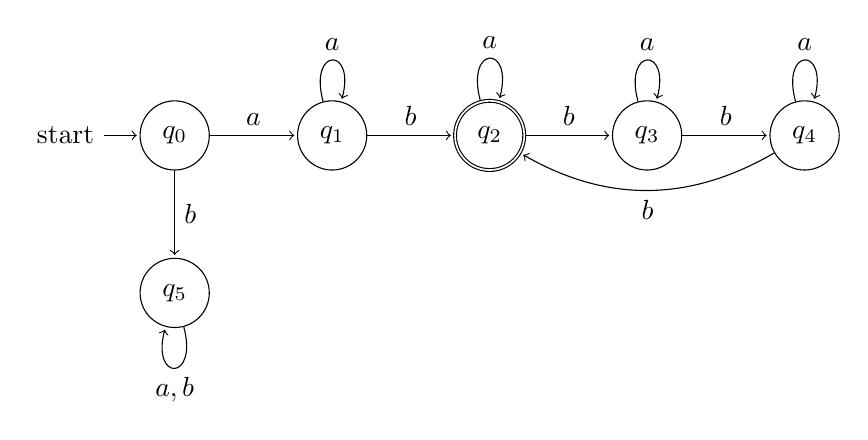
\begin{tikzpicture}[shorten >=1pt,node distance=2cm,on grid,auto] 
                \node[state,initial] (q_0)   {$q_0$}; 
                \node[state] [right=of q_0] (q_1) {$q_1$};
                \node[state,accepting] [right=of q_1] (q_2) {$q_2$};
                \node[state] [right=of q_2] (q_3) {$q_3$};
                \node[state] [right=of q_3] (q_4) {$q_4$};
                \node[state] [below=of q_0] (q_5) {$q_5$};
                \path[->]
                (q_0) 
                edge node {$a$} (q_1)
                edge node {$b$} (q_5)
                (q_1)
                edge [loop above] node {$a$} ()
                edge node {$b$} (q_2)
                (q_2)
                edge [loop above] node {$a$} ()
                edge node {$b$} (q_3)
                (q_3)
                edge [loop above] node {$a$} ()
                edge node {$b$} (q_4)
                (q_4)
                edge [loop above] node {$a$} ()
                edge [bend left, below] node {$b$} (q_2)
                (q_5)
                edge [loop below] node {$a,b$} ();
            \end{tikzpicture}
        \end{center}


    \end{homeworkProblem}
    

    \end{document}